%
% ---------------------------------------------------------------
% Copyright (C) 2012-2018 Gang Li
% ---------------------------------------------------------------
%
% This work is the default powerdot-tuliplab style test file and may be
% distributed and/or modified under the conditions of the LaTeX Project Public
% License, either version 1.3 of this license or (at your option) any later
% version. The latest version of this license is in
% http://www.latex-project.org/lppl.txt and version 1.3 or later is part of all
% distributions of LaTeX version 2003/12/01 or later.
%
% This work has the LPPL maintenance status "maintained".
%
% This Current Maintainer of this work is Gang Li.
%
%

\documentclass[
 size=14pt,
 paper=smartboard,  %a4paper, smartboard, screen
 mode=present, 		%present, handout, print
 display=slides, 	% slidesnotes, notes, slides
 style=tuliplab,  	% TULIP Lab style
 pauseslide,
 fleqn,leqno]{powerdot}


\usepackage{cancel}
\usepackage{caption}
\usepackage{stackengine}
\usepackage{smartdiagram}
\usepackage{attrib}
\usepackage{amssymb}
\usepackage{amsmath} 
\usepackage{amsthm} 
\usepackage{mathtools}
\usepackage{rotating}
\usepackage{graphicx}
\usepackage{boxedminipage}
\usepackage{rotate}
\usepackage{calc}
\usepackage[absolute]{textpos}
\usepackage{psfrag,overpic}
\usepackage{fouriernc}
\usepackage{pstricks,pst-3d,pst-grad,pstricks-add,pst-text,pst-node,pst-tree}
\usepackage{moreverb,epsfig,subfigure}
\usepackage{color}
\usepackage{booktabs}
\usepackage{etex}
\usepackage{breqn}
\usepackage{multirow}
\usepackage{natbib}
\usepackage{bibentry}
\usepackage{gitinfo2}
\usepackage{siunitx}
\usepackage{nicefrac}
%\usepackage{geometry}
%\geometry{verbose,letterpaper}
\usepackage{media9}
\usepackage{animate}
%\usepackage{movie15}
\usepackage{auto-pst-pdf}

\usepackage{breakurl}
\usepackage{fontawesome}
\usepackage{xcolor}
\usepackage{multicol}



\usepackage{verbatim}
\usepackage[utf8]{inputenc}
\usepackage{dtk-logos}
\usepackage{tikz}
\usepackage{adigraph}
%\usepackage{tkz-graph}
\usepackage{hyperref}
%\usepackage{ulem}
\usepackage{pgfplots}
\usepackage{verbatim}
\usepackage{fontawesome}


\usepackage{todonotes}
% \usepackage{pst-rel-points}
\usepackage{animate}
\usepackage{fontawesome}

\usepackage{listings}
\lstset{frameround=fttt,
frame=trBL,
stringstyle=\ttfamily,
backgroundcolor=\color{yellow!20},
basicstyle=\footnotesize\ttfamily}
\lstnewenvironment{code}{
\lstset{frame=single,escapeinside=`',
backgroundcolor=\color{yellow!20},
basicstyle=\footnotesize\ttfamily}
}{}


\usepackage{hyperref}
\hypersetup{ % TODO: PDF meta Data
  pdftitle={Presentation Title},
  pdfauthor={Gang Li},
  pdfpagemode={FullScreen},
  pdfborder={0 0 0}
}


% \usepackage{auto-pst-pdf}
% package to show source code

\definecolor{LightGray}{rgb}{0.9,0.9,0.9}
\newlength{\pixel}\setlength\pixel{0.000714285714\slidewidth}
\setlength{\TPHorizModule}{\slidewidth}
\setlength{\TPVertModule}{\slideheight}
\newcommand\highlight[1]{\fbox{#1}}
\newcommand\icite[1]{{\footnotesize [#1]}}

\newcommand\twotonebox[2]{\fcolorbox{pdcolor2}{pdcolor2}
{#1\vphantom{#2}}\fcolorbox{pdcolor2}{white}{#2\vphantom{#1}}}
\newcommand\twotoneboxo[2]{\fcolorbox{pdcolor2}{pdcolor2}
{#1}\fcolorbox{pdcolor2}{white}{#2}}
\newcommand\vpspace[1]{\vphantom{\vspace{#1}}}
\newcommand\hpspace[1]{\hphantom{\hspace{#1}}}
\newcommand\COMMENT[1]{}

\newcommand\placepos[3]{\hbox to\z@{\kern#1
        \raisebox{-#2}[\z@][\z@]{#3}\hss}\ignorespaces}

\renewcommand{\baselinestretch}{1.2}


\newcommand{\draftnote}[3]{
	\todo[author=#2,color=#1!30,size=\footnotesize]{\textsf{#3}}	}
% TODO: add yourself here:
%
\newcommand{\gangli}[1]{\draftnote{blue}{GLi:}{#1}}
\newcommand{\shaoni}[1]{\draftnote{green}{sn:}{#1}}
\newcommand{\gliMarker}
	{\todo[author=GLi,size=\tiny,inline,color=blue!40]
	{Gang Li has worked up to here.}}
\newcommand{\snMarker}
	{\todo[author=Sn,size=\tiny,inline,color=green!40]
	{Shaoni has worked up to here.}}

%%%%%%%%%%%%%%%%%%%%%%%%%%%%%%%%%%%%%%%%%%%%%%%%%%%%%%%%%%%%%%%%%%%%%%%%
% title
% TODO: Customize to your Own Title, Name, Address
%
\title{Hotel TULIP (a hypothetical organisation)}
\author{
Sarah Sun
\\
\\Deakin University
}
\date{\gitCommitterDate}


% Customize the setting of slides
\pdsetup{
% TODO: Customize the left footer, and right footer
rf=\href{http://www.tulip.org.au}{
Last Changed by: \textsc{\gitCommitterName}\ \gitVtagn-\gitAbbrevHash\ (\gitAuthorDate)
},
cf={Hotel TULIP (a hypothetical organisation)},
}


\begin{document}

\maketitle

%\begin{slide}{Overview}
%\tableofcontents[content=sections]
%\end{slide}


%%==========================================================================================
%%
\begin{slide}[toc=,bm=]{Overview}
\tableofcontents[content=currentsection,type=1]
\end{slide}
%%
%%==========================================================================================


\section{Background}


%%==========================================================================================
%%
\begin{slide}{Hotel TULIP (a hypothetical organisation)}
\begin{center}
\twotonebox{\rotatebox{90}{Defn}}{\parbox{.86\textwidth}
{Special purpose: Not only does it embody all the creative energy.\\ Spirit of TULIP-Lab, it’s a “learning environment” on which the tourism and hospitality students are trained for future hoteliers.
\begin{itemize}
\item \textcolor{orange}{a hypothetical organisations} 
\item A five star hotel that locates in Australia.
\end{itemize}
}}

\end{center}
\bigskip


\end{slide}
%%
%%==========================================================================================


%%==========================================================================================
%%
%%
%%==========================================================================================


%%==========================================================================================
%%
\begin{slide}{Analysis purposes}
\twotonebox {\rotatebox{90}{purposes}}{\parbox{.88\textwidth}
{
Improve their {\textcolor{orange}{potential customers’ online experience},and help their Market Promotion Division to{\textcolor{orange} {identify potential customers and their behaviour patterns}}
\begin{itemize}
\item
In the past two decades.
\item
the Web server of Hotel TULIP has logged all the web traffic to the hotel website.
\item
Stored large amount of data related to the use of various web pages.
\end{itemize}
}
}}


%%==========================================================================================

\end{slide}


\section{ETL}


%%==========================================================================================
%%
\begin{slide}{Extraction}

\begin{itemize}
\item
Existing Methods - \textcolor{orange}{Unzip and read all the network log files}
\item
Count file number-120

\vspace{1cm}
\twocolumn{
	\begin{figure}
		\centering
		\selectcolormodel{rgb}
		%\missingfigure{Testing.}
		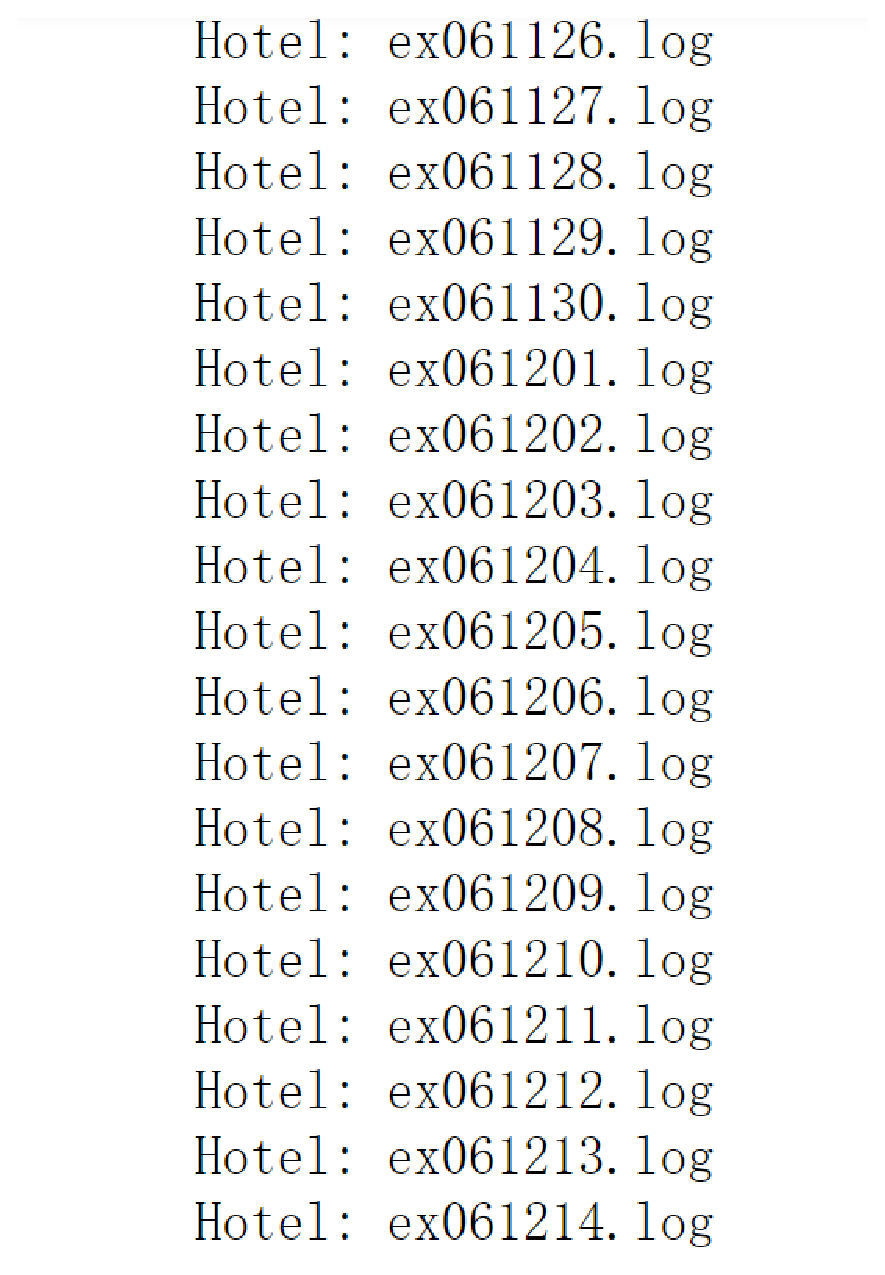
\includegraphics[width=0.6\textwidth]{Capture.eps}\\
		\caption{loading}\label{fig:loading}
	\end{figure}
}{
	\begin{figure}
		\centering
		\selectcolormodel{rgb}
		%\missingfigure{Testing.}
	    
\includegraphics[width=0.6\textwidth]{Capture1.eps}\\
		\caption{numbers}\label{fig:timg}
	\end{figure}
}
\end{itemize}

\end{slide}
%%
%%==========================================================================================


%%==========================================================================================
%%
\begin{slide}[toc=,bm=]{Loading data}

\begin{itemize}
\item
Print the first five lines to view the data in general form
\begin{figure}
	\centering
	\selectcolormodel{rgb}
	%\missingfigure{Testing.}
	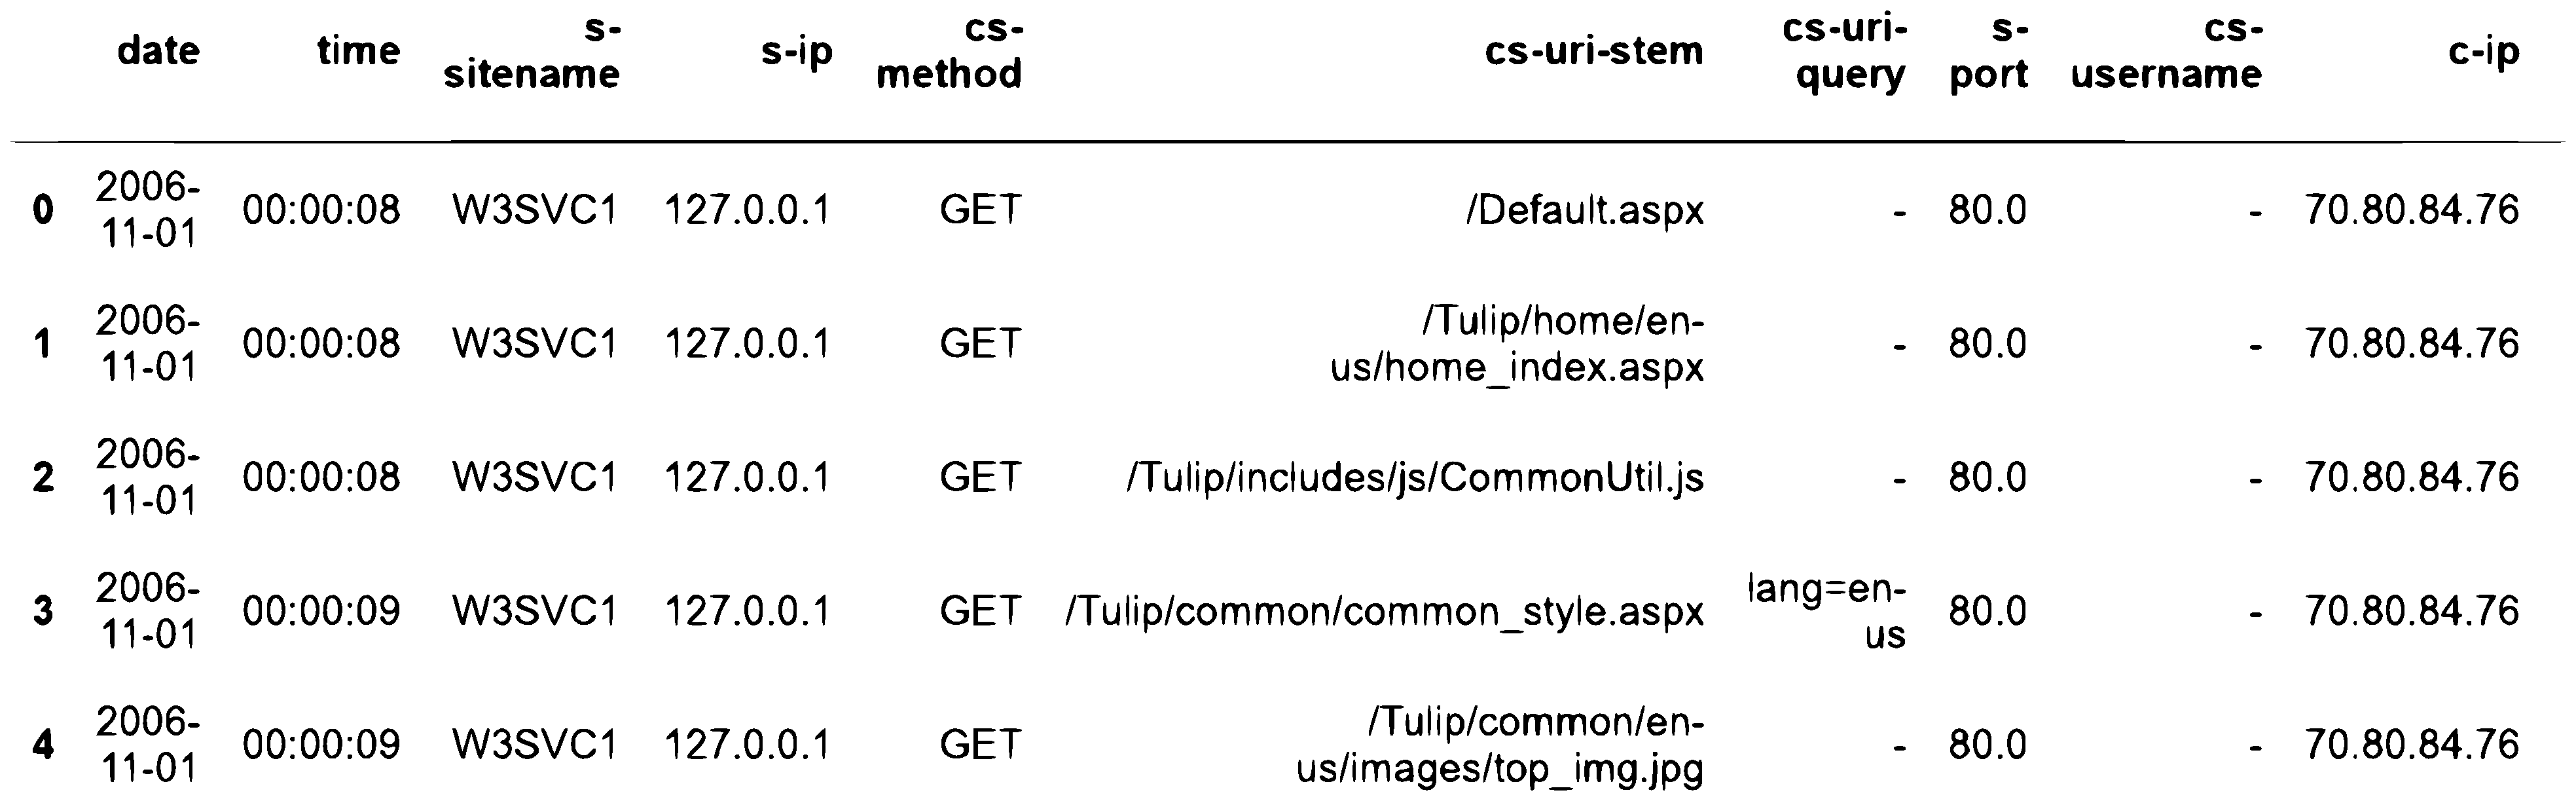
\includegraphics[width=0.6\textwidth]{Capture2.eps}\\
	\caption{head}\label{fig:timg}
\end{figure}
\begin{figure}
	\centering
	\selectcolormodel{rgb}
	%\missingfigure{Testing.}
	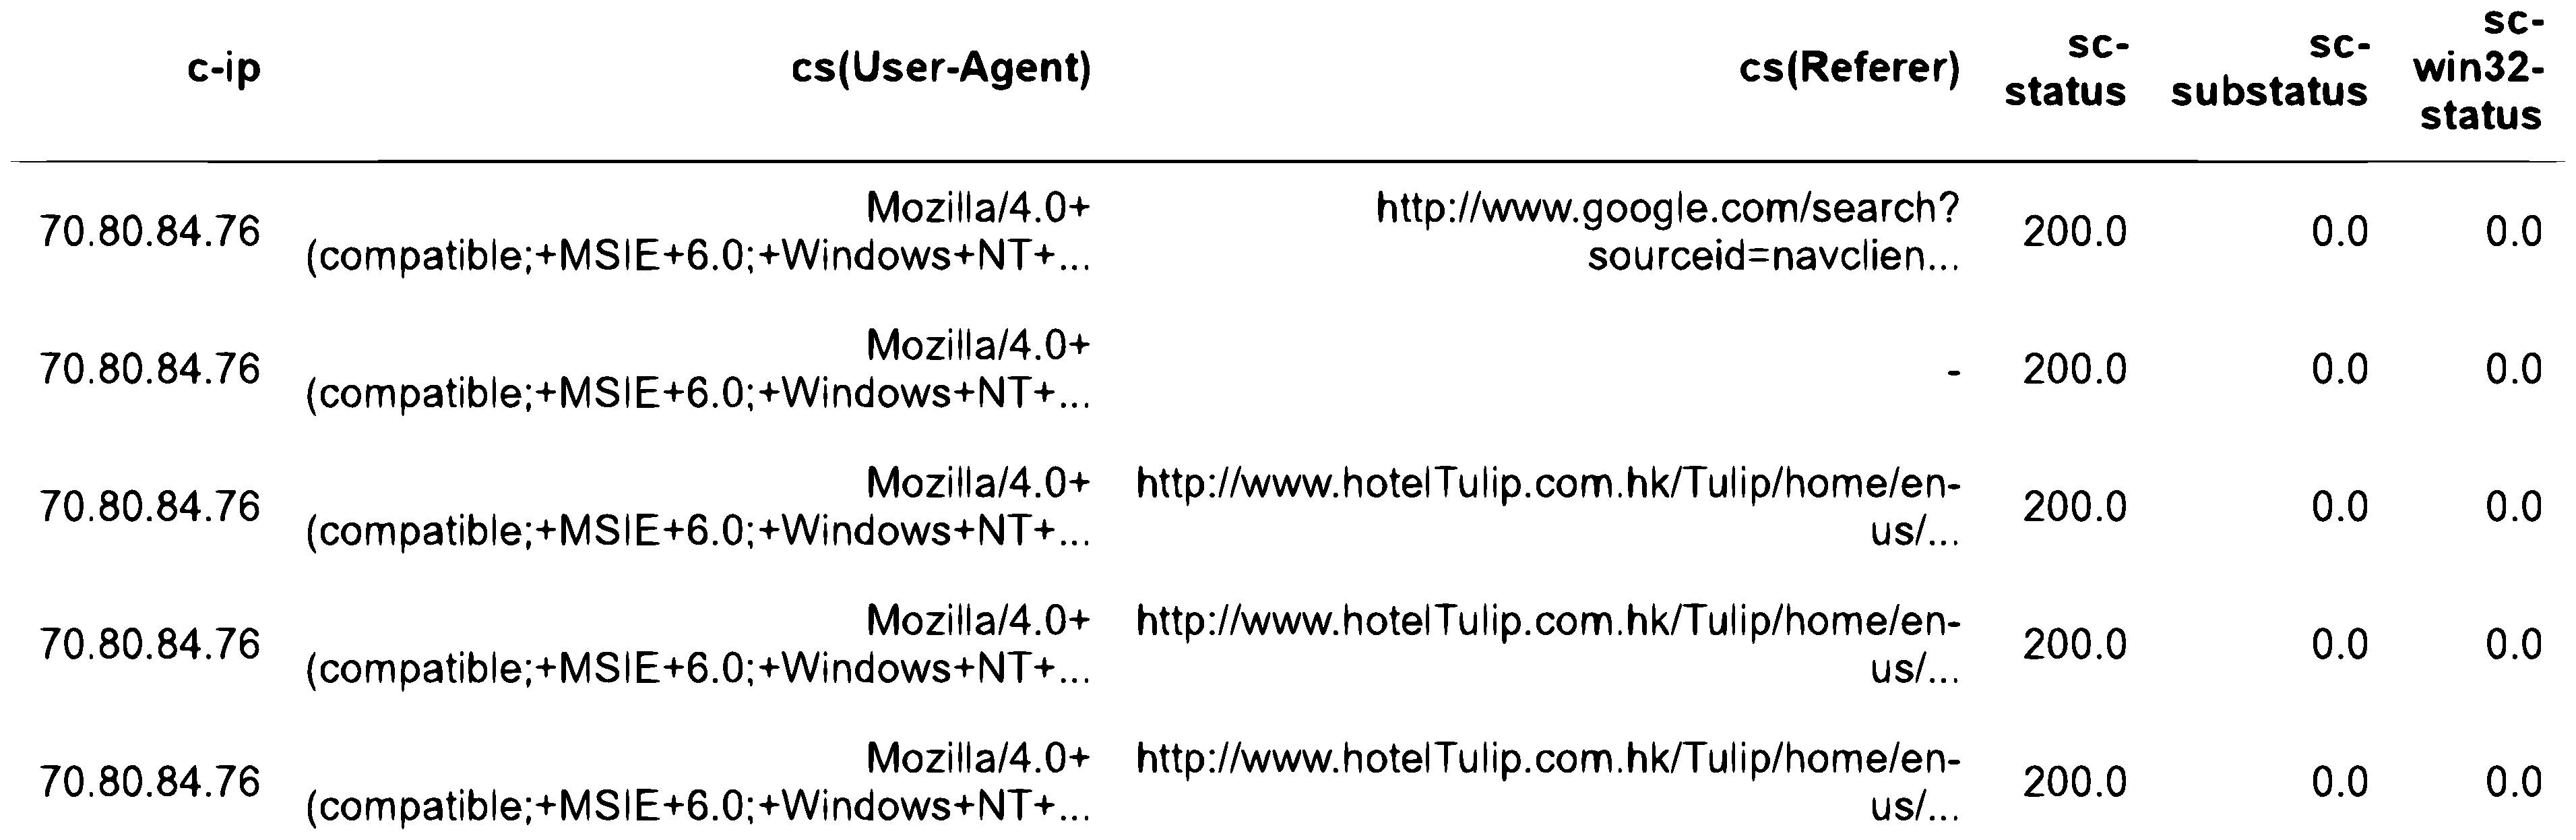
\includegraphics[width=0.6\textwidth]{Capture3.eps}\\
	\caption{head}\label{fig:timg}
\end{figure}
\end{itemize}

\end{slide}
%%
%%==========================================================================================


%%==========================================================================================
%%
\begin{slide}[toc=,bm=]{Data attribute}
\begin{figure}
	\centering
	\selectcolormodel{rgb}
	%\missingfigure{Testing.}
	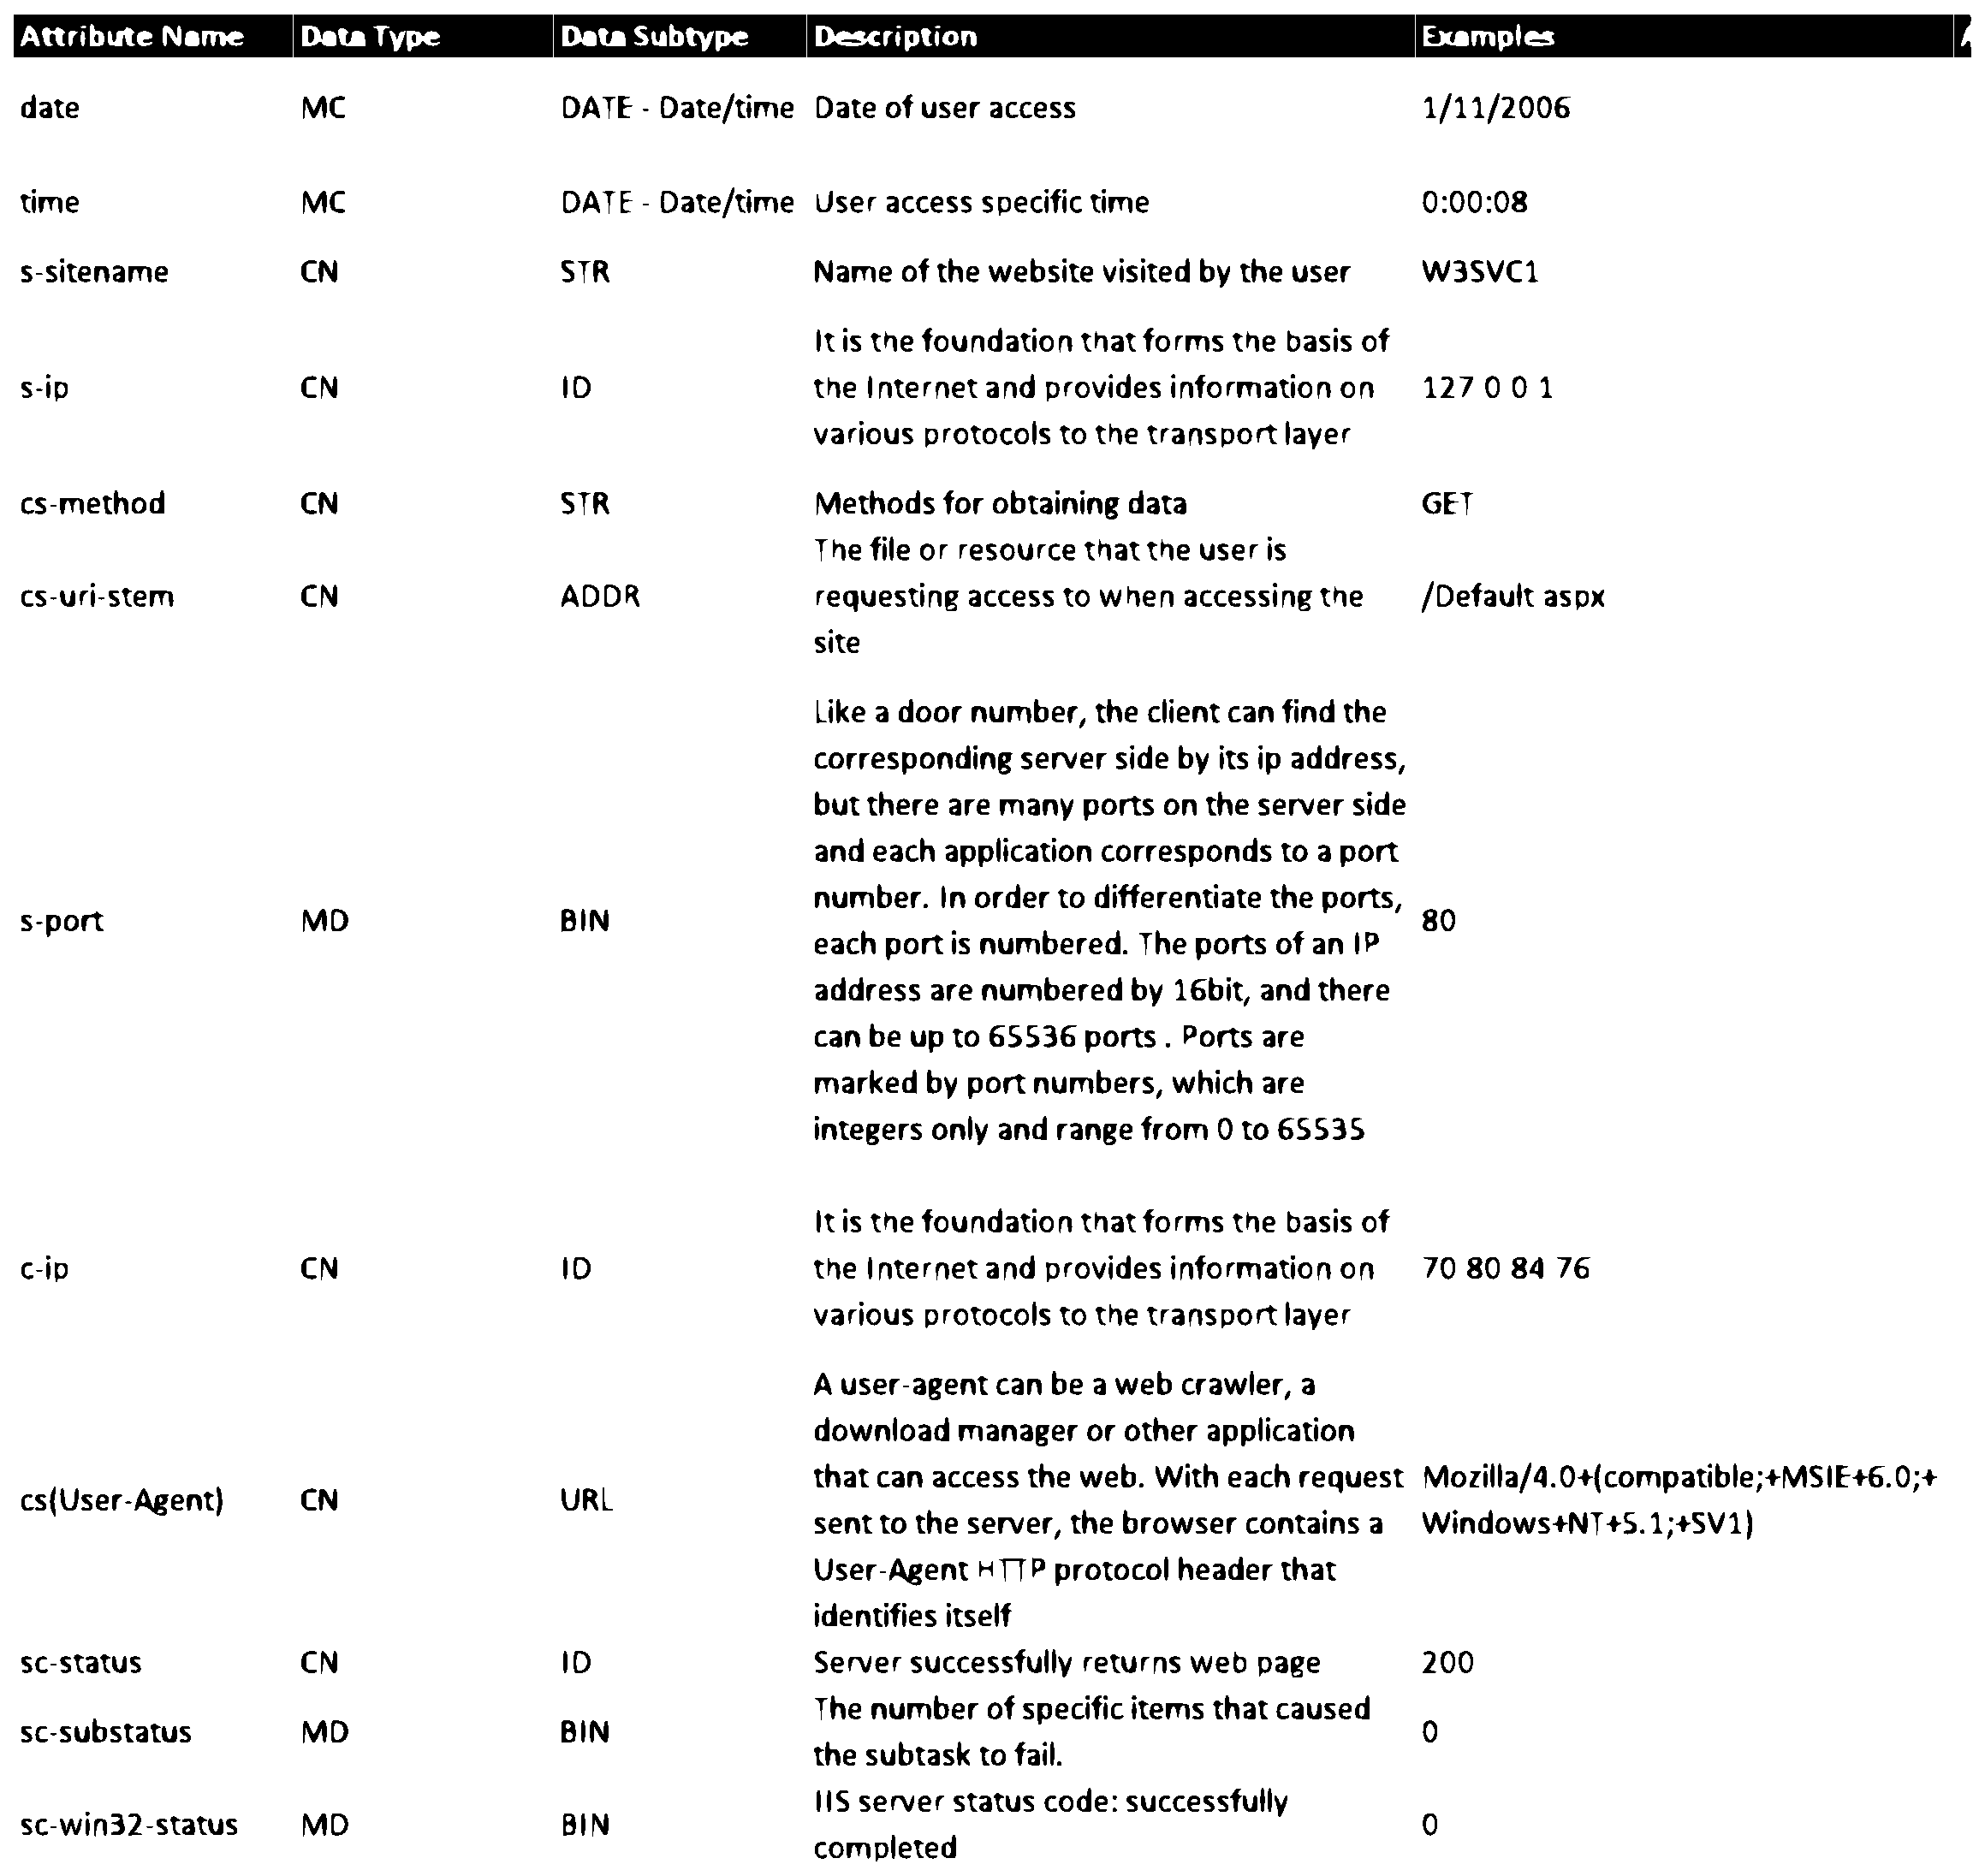
\includegraphics[width=0.6\textwidth]{Capture4.eps}\\
	\caption{attribute }\label{fig:timg}
\end{figure}
\end{slide}

%%
\begin{slide}{Data cleaning}
\begin{itemize}
\item
Calculates NaN for rows and columns in the data
\item
After cleaning up more than 15 percent of the columns, remove the rows with NaN
\end{itemize}
\vspace{1cm}
\twocolumn{
	\begin{figure}
		\centering
		\selectcolormodel{rgb}
		%\missingfigure{Testing.}
		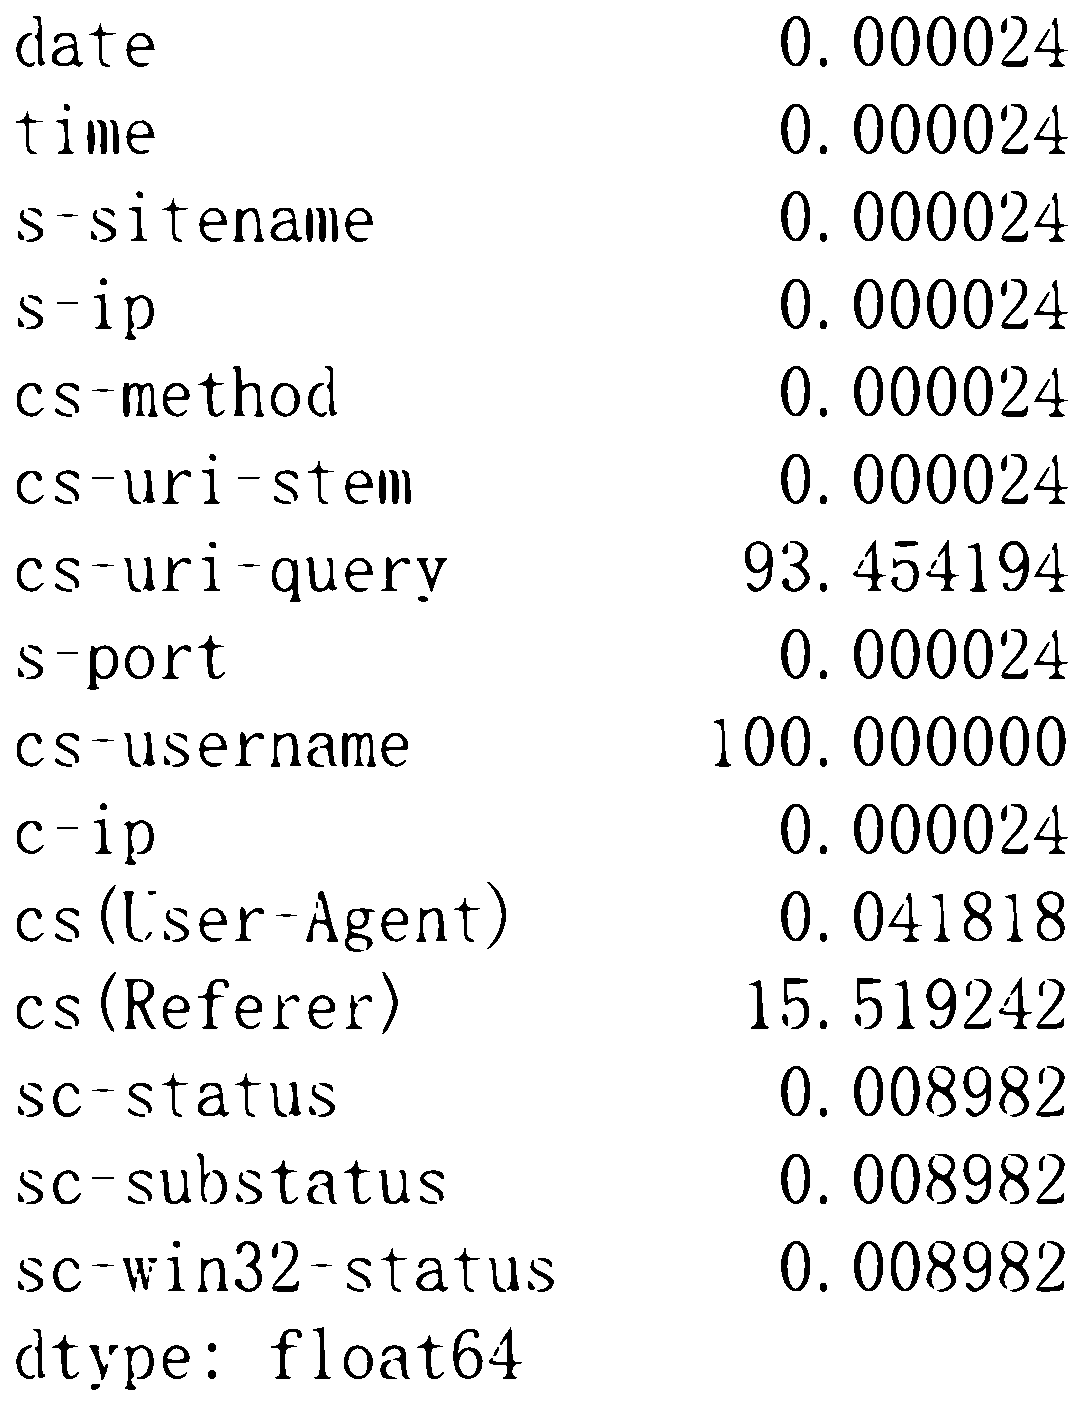
\includegraphics[width=0.6\textwidth]{Capture5.eps}\\
		\caption{Cleaning >=15\% data}\label{fig:loading}
	\end{figure}
}{
\begin{figure}
	\centering
	\selectcolormodel{rgb}
	%\missingfigure{Testing.}
	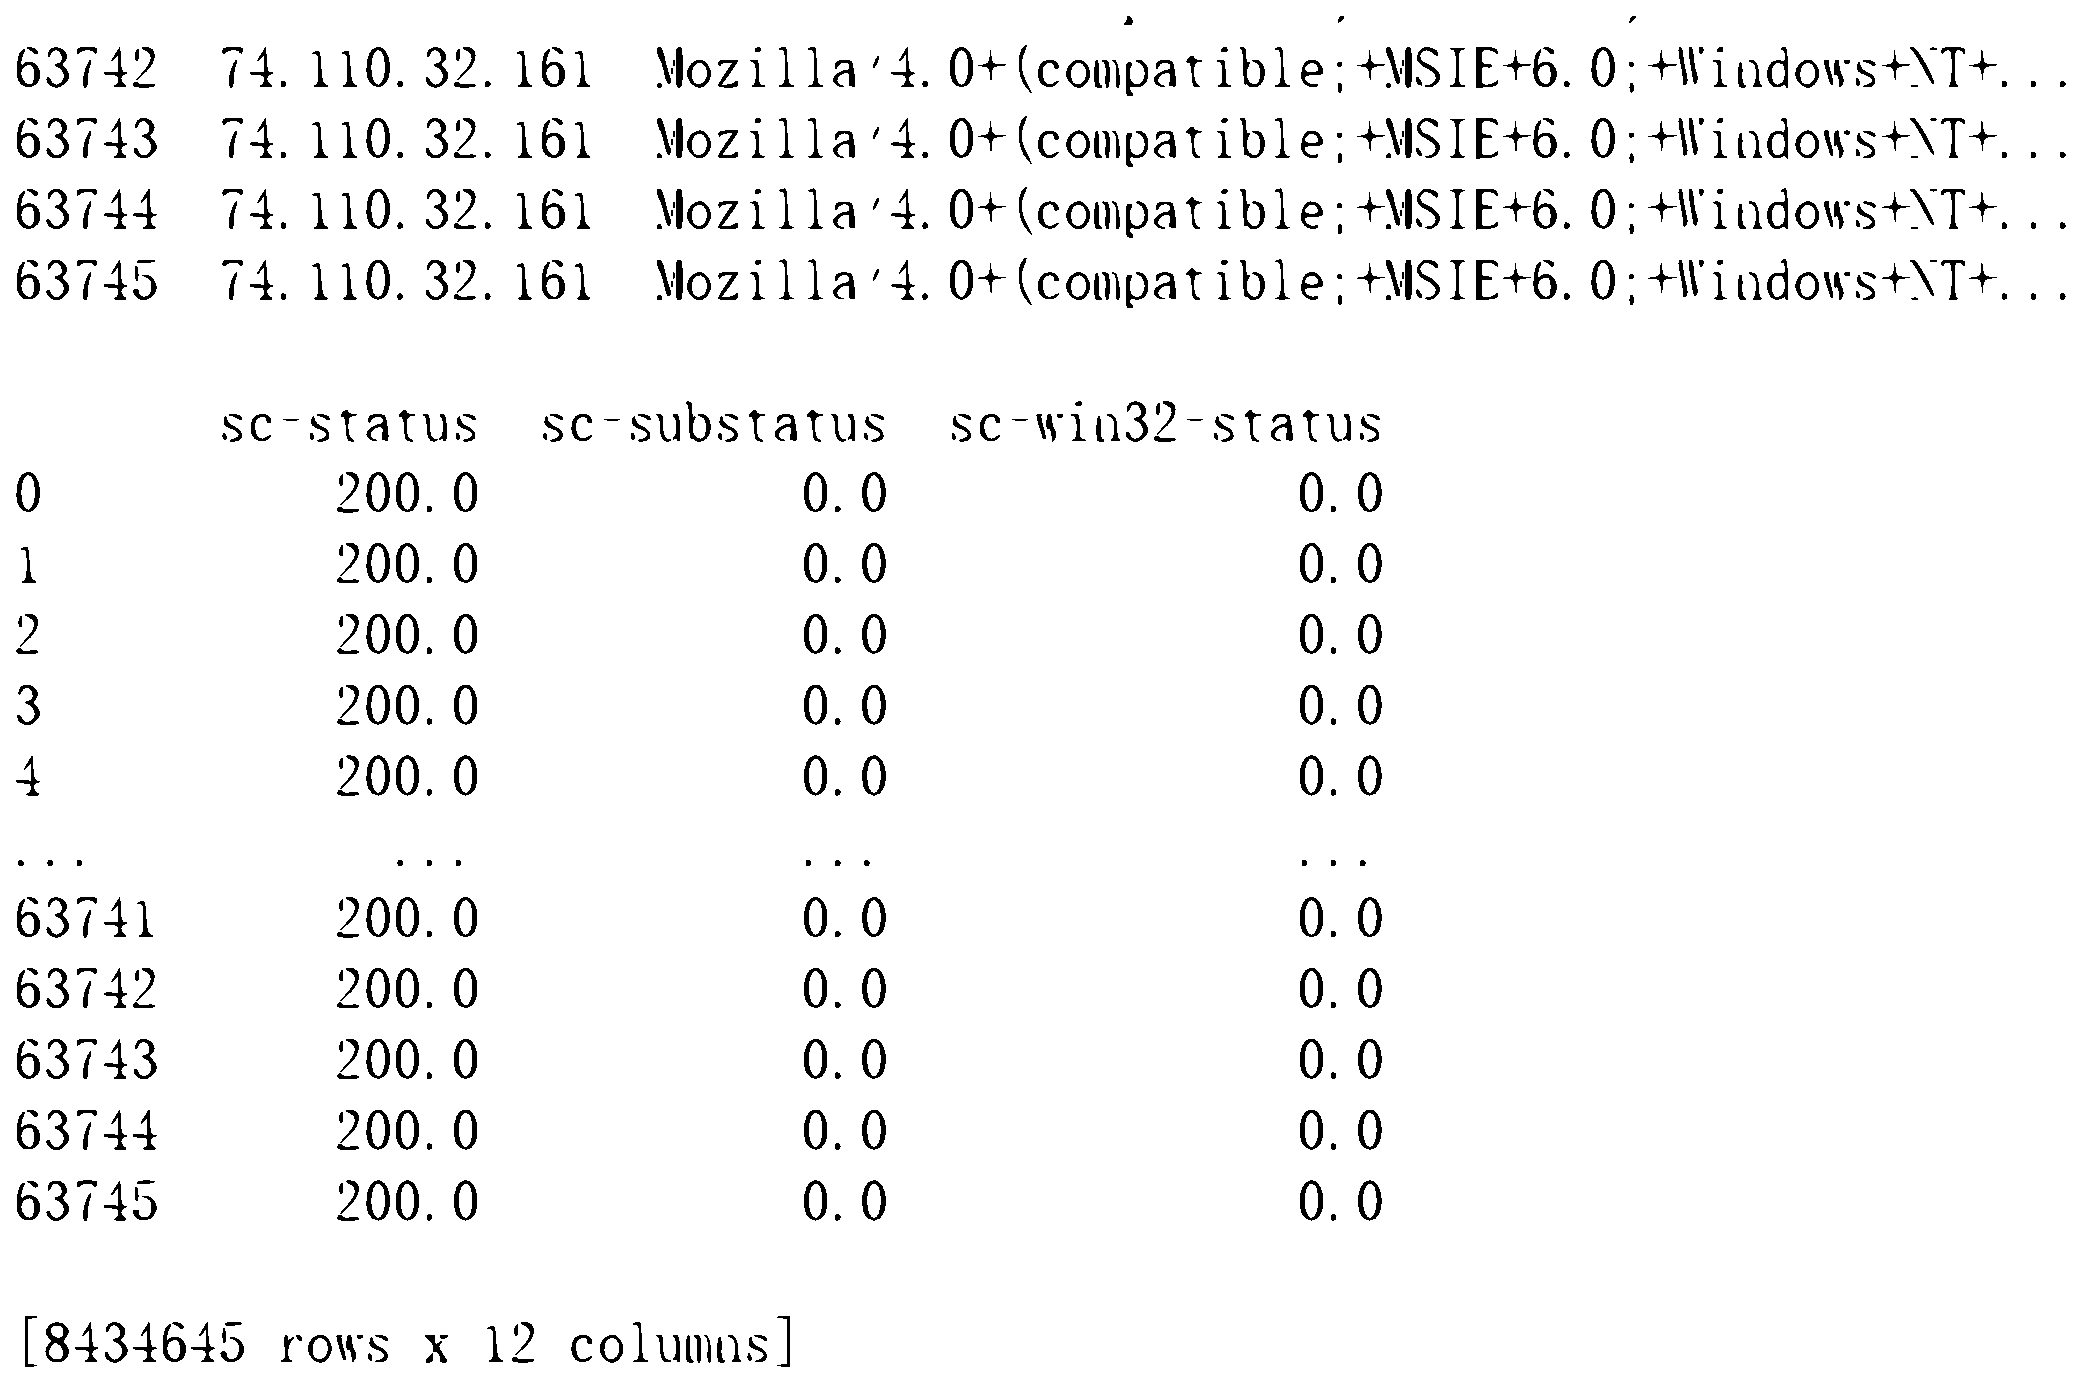
\includegraphics[width=1\textwidth]{Capture6.eps}\\
	\caption{Finished cleaning 8434645 rows}\label{fig:loading}
\end{figure}
}

\end{slide}
%%

\section{Data Statistics Description}


%%==========================================================================================
%%
\begin{slide}{Step One - Traffic Analysis}
\begin{itemize}
\item
\smallskip
All data from 2006 to 2007 are broken down by hour, from 0:00 to 23:00, with traffic analysis for each hour.
\end{itemize}

\begin{figure}[htbp]
    \centering
    \subfigure[traffic analysis]{
        \selectcolormodel{rgb}
       % \missingfigure[figwidth=5.5cm]{Test.}
        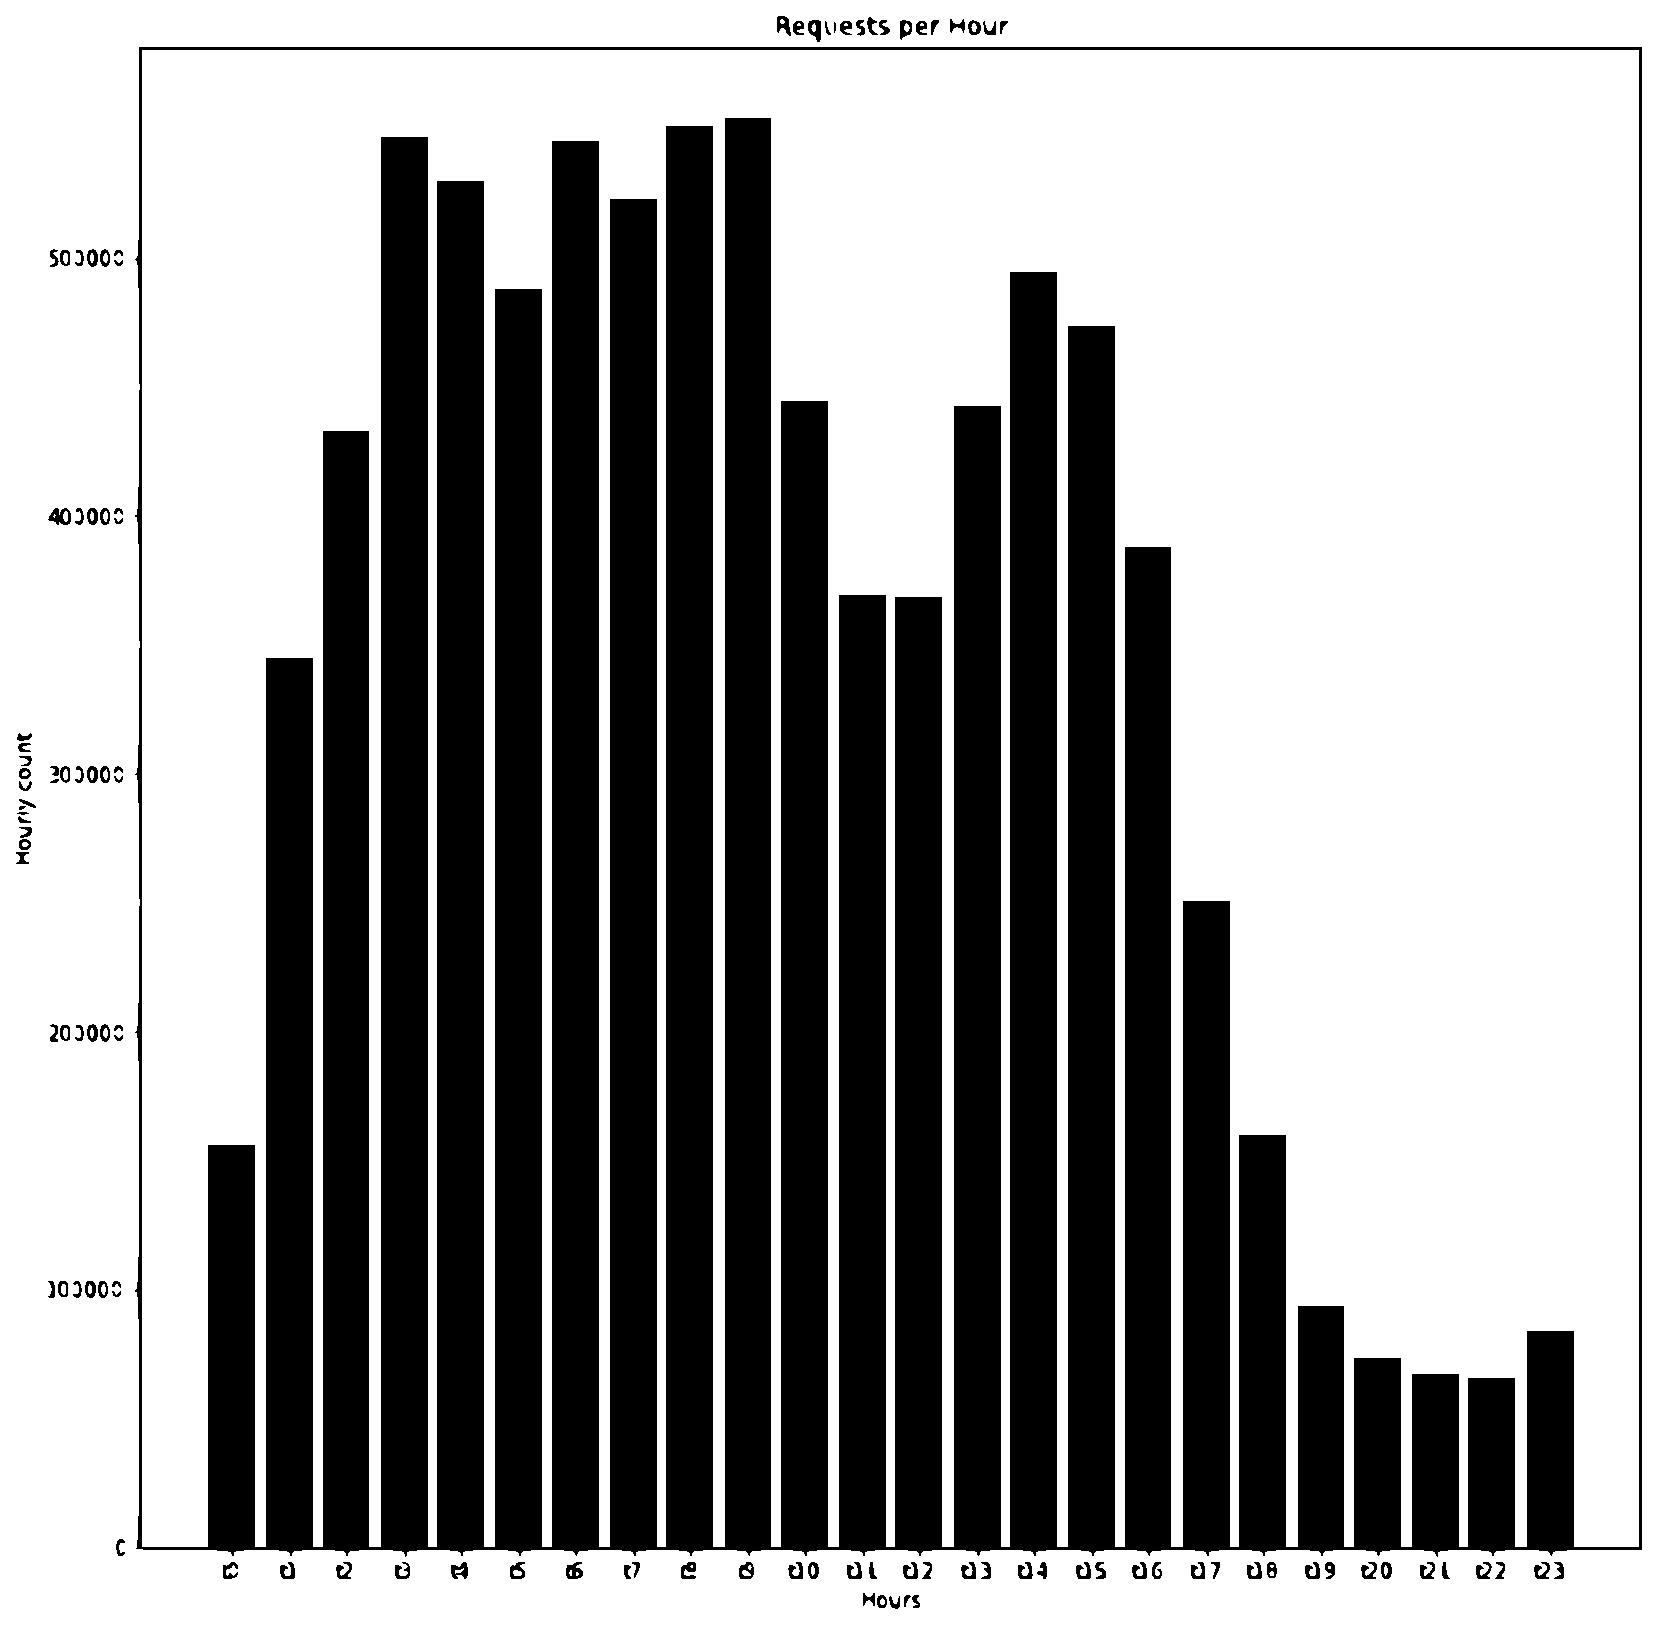
\includegraphics[width=0.4\textwidth]{ll1.eps}
        \label{traffic analysis}
    }
\end{figure}

\end{slide}
%%
%%==========================================================================================


%%==========================================================================================
%%
\begin{slide}{Step two: Server Analysis}
\begin{figure}[htbp]
	\centering
	\subfigure[traffic analysis]{
		\selectcolormodel{rgb}
		% \missingfigure[figwidth=5.5cm]{Test.}
		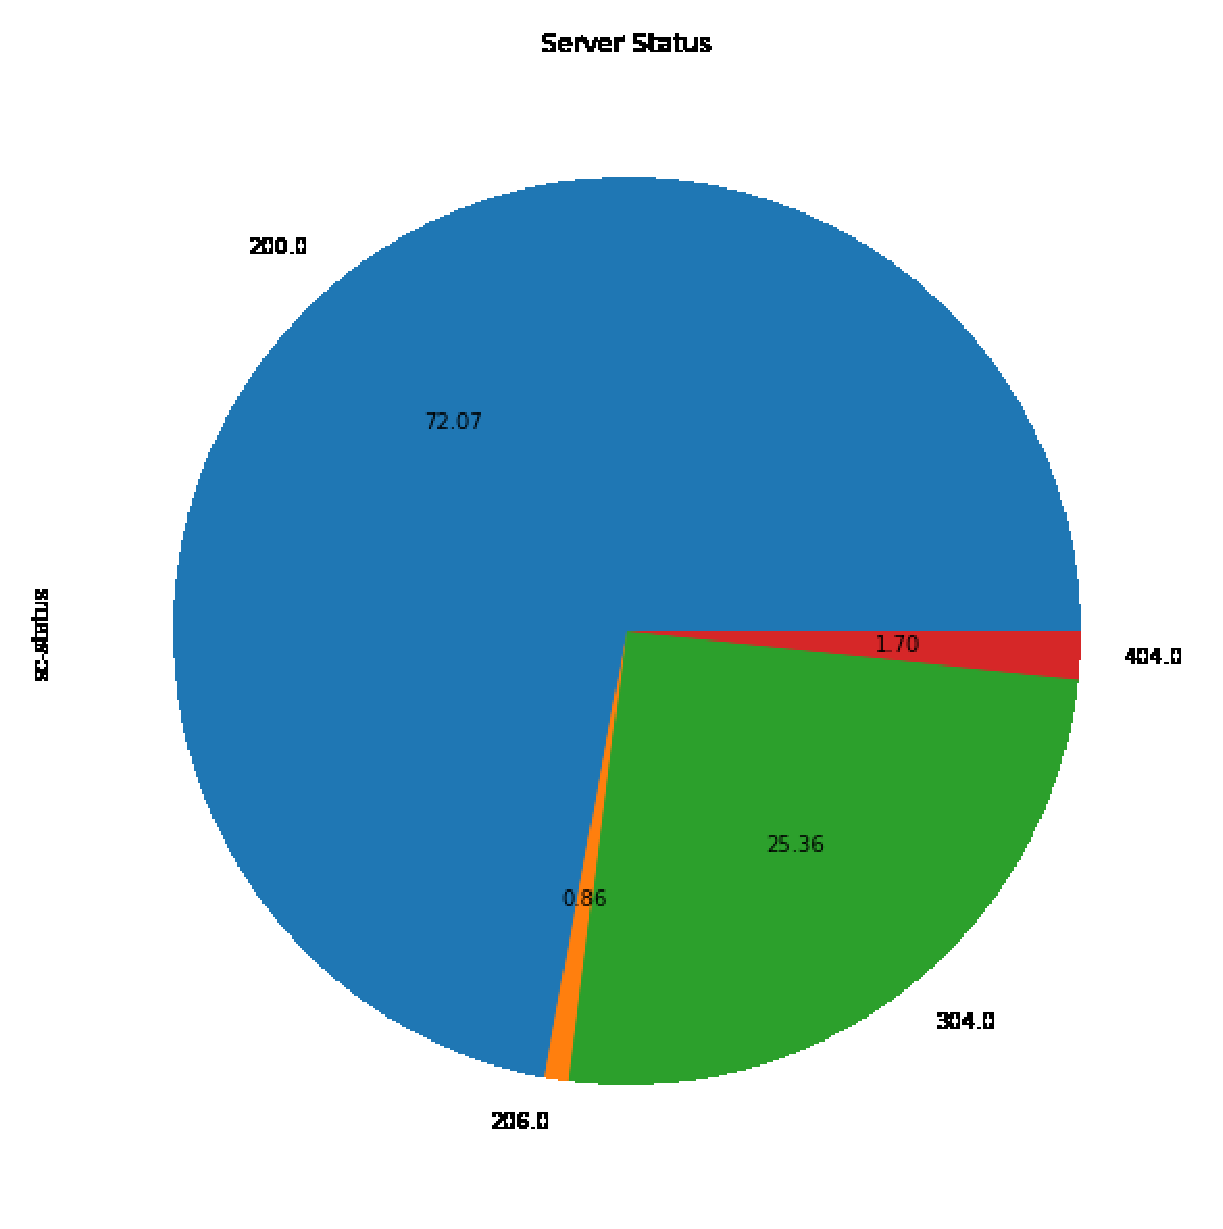
\includegraphics[width=0.5\textwidth]{ll2.eps}
		\label{server analysis}
	}
\end{figure}

%%====================================================================
\end{slide}
%%
%%==========================================================================================

\section{Geographic Analysis}


%%==========================================================================================
%%
\begin{slide}[toc=,bm=]{Country}
\begin{figure}[htbp]
	\centering
	\subfigure[traffic analysis]{
		\selectcolormodel{rgb}
		% \missingfigure[figwidth=5.5cm]{Test.}
		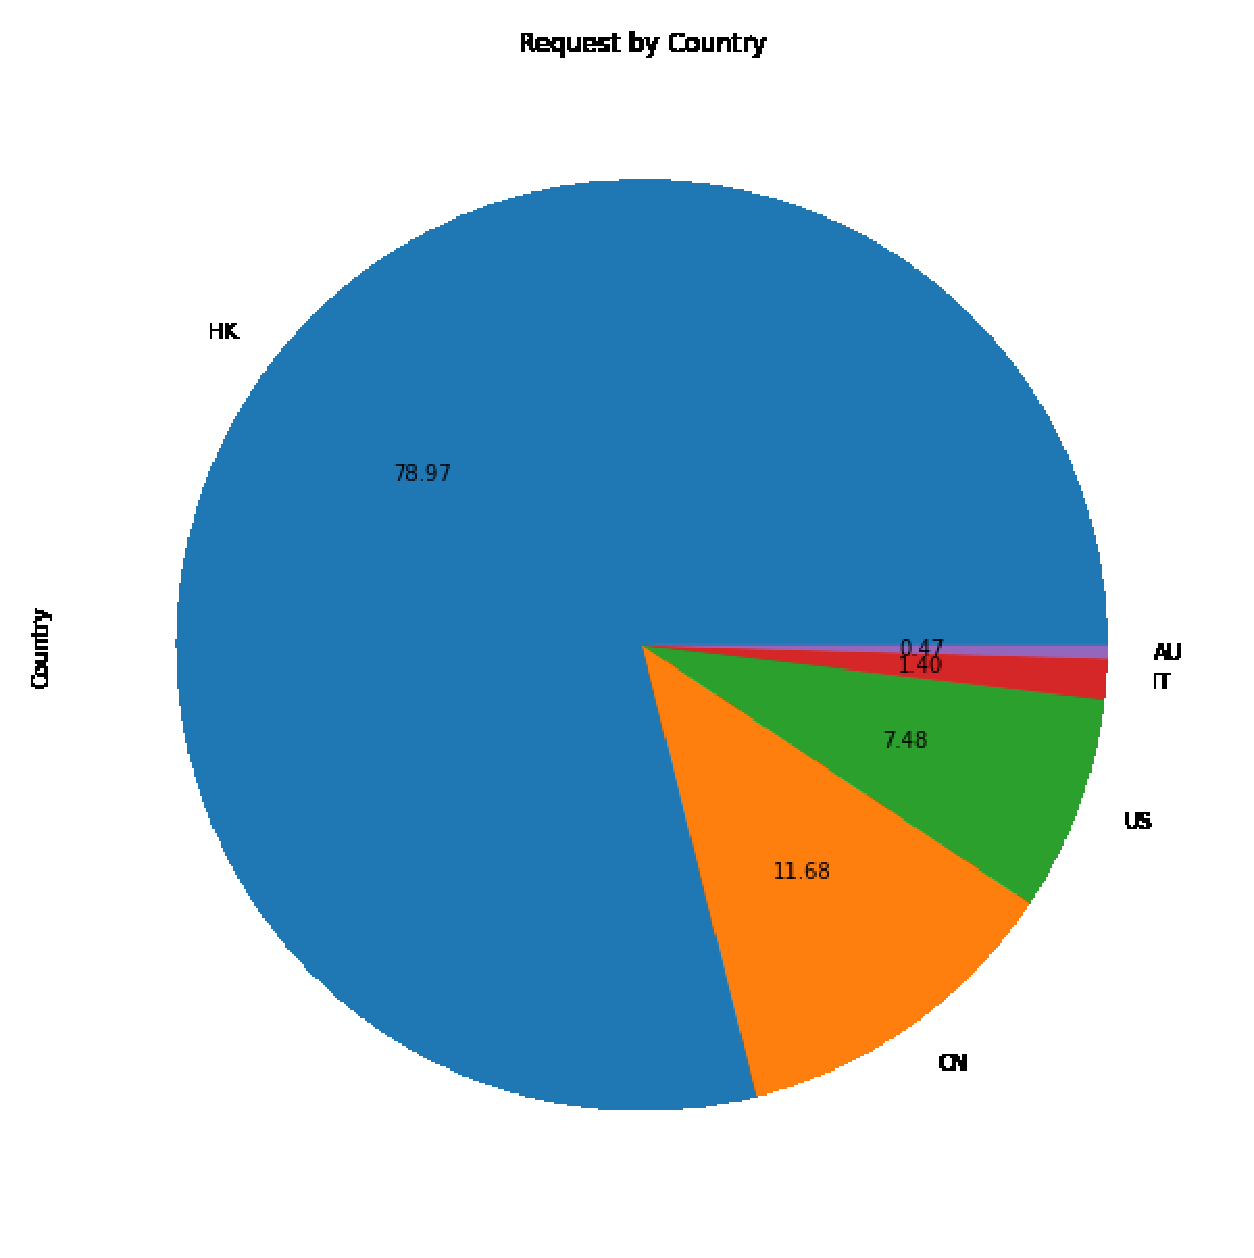
\includegraphics[width=0.6\textwidth]{ll3.eps}
		\label{Country}
	}
\end{figure}
\end{slide}
%%
%%
\begin{slide}{City}
\begin{figure}[htbp]
	\centering
	\subfigure[traffic analysis]{
		\selectcolormodel{rgb}
		% \missingfigure[figwidth=5.5cm]{Test.}
		\includegraphics[width=0.6\textwidth]{ll4.eps}
		\label{City}
	}
\end{figure}


\end{slide}

\section{Conclusion}

%%==========================================================================================
%%
\begin{slide}[toc=,bm=]{Conclusion}
\begin{itemize}
\item
\smallskip
The overall idea: decompress the dataset, load it, read it. And clean up any unnecessary data in it, such as nan, - or spaces.

\item
\smallskip
Three aspects of the data were visualised for the data.\\

By using bar charts and pie charts to analyse when web traffic is concentrated and the corresponding situation on the website, and finally by city and country, to compare the countries and cities with the highest number of visitors.

\end{itemize}

%%==========================================================================================


\end{slide}
%%
%%==========================================================================================


%%==========================================================================================
%
\begin{slide}[toc=,bm=]{Questions?}
\begin{center}
\begin{figure}
    \animategraphics[autoplay, loop, height=0.4\textheight]{5}{figures//gif//question//q_}{1}{30}
\end{figure}
\end{center}
\end{slide}
%%
%%==========================================================================================


%%==========================================================================================
% TODO: Contact Page
\begin{wideslide}[toc=,bm=]{Contact Information}
\centering
\vspace{\stretch{1}}
\twocolumn[
lcolwidth=0.35\linewidth,
rcolwidth=0.65\linewidth
]
{
% \centerline{\includegraphics[scale=.2]{tulip-logo.eps}}
}
{
\vspace{\stretch{1}}
 Fresh Fish: Sarah Sun\\
Deakin University, Australia
\begin{description}
 \item[\textcolor{orange}{\faEnvelope}] \href{mailto:sunhan@deakin.edu.au}
 {\textsc{\footnotesize{sunhan@deakin.edu.au}}}

 \item[\textcolor{orange}{\faHome}] \href{http://www.tulip.org.au}
 {\textsc{\footnotesize{group 00}}}
\end{description}
}
\vspace{\stretch{1}}
\end{wideslide}

\end{document}

\endinput
